\documentclass[aspectratio=169,xcolor={svgnames,table},10pt,fleqn]{beamer}
\usepackage{stb-beamer-a}

%---- AMS math ---------------------------------------------------------
\usepackage{amsmath,amsthm}

%---- Fonts ------------------------------------------------------------
\usefonttheme{professionalfonts}

\usepackage[T1]{fontenc}
\usepackage{textcomp}
\usepackage[default,medium,scaled=1.0]{raleway}
\usepackage[scaled=0.80]{arevmath}

%---- Packages ---------------------------------------------------------

\usepackage{tikz}
\usetikzlibrary{positioning,arrows.meta,shapes.geometric}
\usepackage{pgfplots}
\usepackage{booktabs}
\usepackage{siunitx}
\cmidrulewidth=\heavyrulewidth

\graphicspath{{figs/}}

%---- Title page -------------------------------------------------------

\title[\footnotesize Journal Club]
      {\Large Bone fracture healing under Ilizarov fixator: Influence of fixator configuration, fracture geometry, and loading}
%\subtitle{}

\author{Philip Frederik Ligthart}
\institute{\itshape Dept of Mech \& Mechatronic Eng,\\
           Stellenbosch University, South Africa}

\date{}

\def\titlefig{\includegraphics[height=5cm]{Figs/Front_two_pages}}

%====================================================================
\begin{document}
\begin{frame}
  \maketitle
\end{frame}

\section{Necessary background}

  \begin{frame}
    \frametitle{Bone fracture healing}
    \begin{columns}
    \column{0.5\textwidth}
      \textbf{Primary bone healing}
      \begin{itemize}
        \item Every day process
        \item Requires absolute stability
      \end{itemize}
    \column{0.5\textwidth}
      \textbf{Secondary bone healing}
      \begin{itemize}
        \item Occurs with relative stability
        \item Involves callus formation - new bone
      \end{itemize}
    \end{columns}
    \vspace{1cm}
    \begin{columns}
      \column{0.5\textwidth}
      \begin{itemize}
        \item Plate fixation
        \item Intramedullary nailing
      \end{itemize}
      \column{0.5\textwidth}
      \begin{itemize}
        \item External fixation
      \end{itemize}
    \end{columns}
  \end{frame}

  \begin{frame}
    \frametitle{Secondary bone healing}
    \begin{itemize}
      \item Bone ends are not in direct contact
      \item Relative motion between bone ends - Interfragmentary movement (IFM)
      \item Bone healing is influenced (theories) by Interfragmentary strain (IFS)
      \vspace{1cm}
      \item Found 10 different mechanoregulation measures in literature
    \end{itemize}
    \vspace{1cm}
    Generally, \qtyrange[range-phrase = --, range-units = single]{2}{10}{\percent} engineering strain is desired
  \end{frame}

  \begin{frame}
    \frametitle{Ilizarov fixator}
    \begin{columns}
      \column{0.5\textwidth}
      \begin{itemize}
        \item Circular rings
        \item Tensioned wires - k-wires - \qtyrange[range-phrase = --, range-units = single]{1.5}{1.8}{\milli\meter}
        \item Half pins - Schanz screws - \qtyrange[range-phrase = --, range-units = single]{3}{6}{\milli\meter}
        \item Threaded rods
      \end{itemize}
      \column{0.5\textwidth}
      \centering
      \textbf{Taylor Spatial Frame (TSF)}
      \includegraphics[height=6cm]{Figs/FEM_model_a.png}
    \end{columns}
  \end{frame}

\section{Talk focus}

  \begin{frame}
    \frametitle{Focus of the talk}
    % Create a flow chart with three side by side boxes each containing a label and arrows from left to right
    \begin{center}
      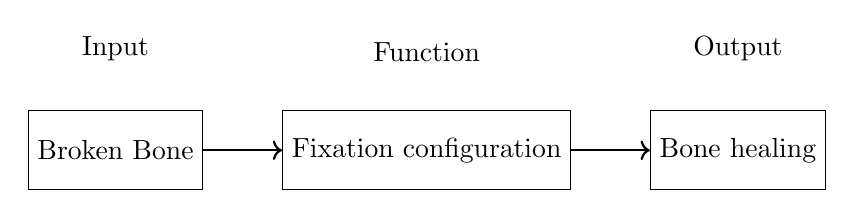
\begin{tikzpicture}
        \node[draw,rectangle,minimum width=2cm,minimum height=1cm] (A) {Broken Bone};
        \node[above=0.5cm of A] {Input};
        \node[draw,rectangle,minimum width=2cm,minimum height=1cm,right=of A] (B) {Fixation configuration};
        \node[above=0.5cm of B] {Function};
        \node[draw,rectangle,minimum width=2cm,minimum height=1cm,right=of B] (C) {Bone healing};
        \node[above=0.5cm of C] {Output};
        \draw[thick,->] (A) -- (B);
        \draw[thick,->] (B) -- (C);
      \end{tikzpicture}
    \end{center}
  \end{frame}

\section{General model}

  \begin{frame}
    \frametitle{General model setup}
    The same general model setup was used simulation and experimental validation
    \begin{itemize}
      \item CT scan of a human tibia used
      \item Perpendicular k-wires
      \item Strut angle of \qty{65}{\degree} remained constant
      \item Bones centred in the rings
    \end{itemize}
  \end{frame}

\section{Numerical model}

  \begin{frame}
    \frametitle{Finite element model}
    \begin{columns}
      \column{0.5\textwidth}
      \begin{itemize}
        \item Homogeneous, linear elastic material properties
        \item Axial load applied as a point load
        \item Geometric non-linearity included for strain stiffening of k-wires
        \item Bone k-wire interface modelled using RBE2 elements (or equivalent)
      \end{itemize}
      \column{0.5\textwidth}
      \centering
      \includegraphics[height=6cm]{Figs/FEM_model_b.png}
    \end{columns}
  \end{frame}

  \begin{frame}
    \frametitle{Finite element parameters}
    \begin{itemize}
      \item COMSOL Multiphysics used for the simulations
      \item Second order tetrahedral elements - all parts
      \item $\approx$ \qty{215000}{elements}
      \item Convergence criteria:
        \begin{itemize}
          \item \qty{0.1}{\milli\meter} for displacement (Absolute)
        \end{itemize}
      \item Mesh convergence study
        \begin{itemize}
          \item $\le\qty{2}{\percent}$ difference between meshes considered converged 
        \end{itemize}
    \end{itemize}
  \end{frame}

\section{Validation}

  \begin{frame}
    \frametitle{Validation}
    \centering
    \includegraphics[height=6cm]{Figs/Validation}
    \begin{itemize}
      \item Used the ARAMIS DIC system to measure displacements.
      \item Quote accuracy of \qty{0.0002}{\milli\meter}
    \end{itemize}
  \end{frame}

  \begin{frame}
    \frametitle{\qty{130}{\milli\meter} ring}
    \centering
    \includegraphics[height=6cm]{Figs/130mm_results}
  \end{frame}

  \begin{frame}
    \frametitle{\qty{155}{\milli\meter} ring}
    \centering
    \includegraphics[height=6cm]{Figs/155mm_results}
  \end{frame}

\section{Parametric study}

  \begin{frame}
    \frametitle{Parameters}
    \begin{table}
      \begin{tabular}{lll}
        \toprule
        Count & Parameter & Variations \\
        \midrule
        2 & Ring diameter & \qtylist[list-units = single]{130;155}{\milli\meter} \\
        3 & K-wire tension & \qtylist[list-units = single]{50;90;130}{\kilo\gram} \\
        3 & Gap size & \qtylist[list-units = single]{1;3;5}{\milli\meter} \\
        3 & Axial load & \qtylist[list-units = single]{100;150;200}{\kilo\gram} \\
        \bottomrule
      \end{tabular}
    \end{table}
    \vspace{1cm}
    Factorial design: $2 \times 3 \times 3 \times 3 = 54$\\
    However: \num{18} simulations were performed
  \end{frame}

\section{Insights}

  \begin{frame}
    \frametitle{Insights}
    \begin{itemize}
      \item Found that out of plane motion/torsion is negligible
      \item Gap size is by far the most influential parameter
    \end{itemize}
  \end{frame}

  \begin{frame}
    \frametitle{Shortcomings}
    \begin{itemize}
      \item Previous authors have found slipping between bone and k-wire -- not considered
      \item Loading limits results -- could explain the lack of out of plane motion
      \item Previous authors have shown yielding of k-wires -- not considered
      \item Output measure is not clear -- measurable IFM or IFS would be more interpretable
      \item Increasing stiffness of callus region not considered
    \end{itemize}
  \end{frame}

\end{document}
